% Chapter Template

\chapter{Ensayos y Resultados} % Main chapter title

\label{Chapter4} % Change X to a consecutive number; for referencing this chapter elsewhere, use \ref{ChapterX}

%----------------------------------------------------------------------------------------
%	SECTION 1
%----------------------------------------------------------------------------------------

%\section{Pruebas funcionales del hardware}
%\label{sec:pruebasHW}

%La idea de esta sección es explicar cómo se hicieron los ensayos, qué resultados se obtuvieron y analizarlos.

\section{Verificación del análisis automático de redes ferroviarias}
	
	Para verificar el correcto funcionamiento del análisis automático de las redes ferroviarias se generaron varias topologías distintas, entre ellas: estaciones simples, estaciones complejas, bypass, playa de maniobras y aleatorias. Para todas ellas se generó automáticamente una tabla de enclavamientos, las cuales fueron comparadas con tablas de enclavamientos realizadas de la forma tradicional por el Ingeniero Ramiro Ghignone de la UTN Facultad Regional Haedo.
	
	En la figura \ref{fig:Mapa_0} se presenta una topología creada aleatoriamente con diversos elementos tales como cambios en cruceta (nodos 14 a 17), bypass (entre los nodos 2-5 y 21-22) y ramificaciones complejas (nodos 2, 5 y 9) de una playa de maniobras hacia un posible taller ferroviario (nodo 13).
	
	\begin{figure}[h]
	\centering
	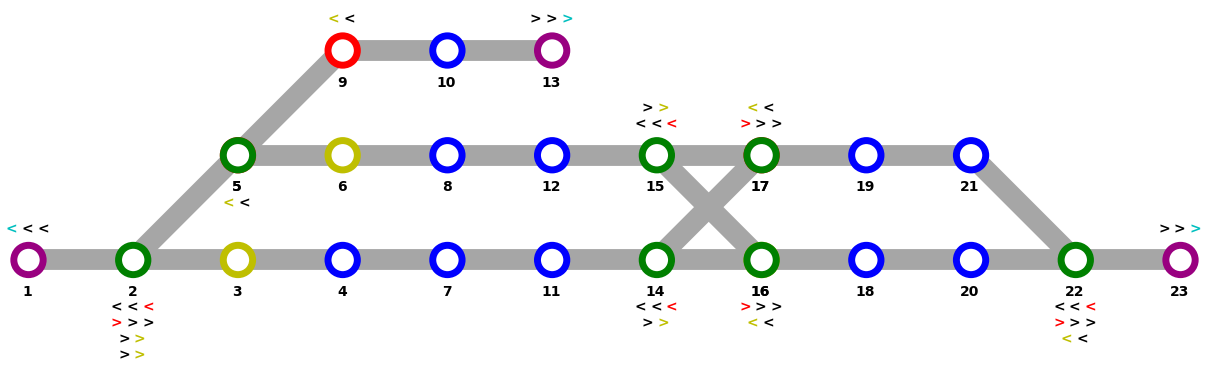
\includegraphics[scale=0.45]{./Figures/Mapa_0}
		\caption{Topología aleatoria generada para probar el análisis automático de redes ferroviarias.}
		\label{fig:Mapa_0}
	\end{figure}
	
	La tabla de enclavamientos generada automáticamente mediante el analizador de redes ferroviarias desarrollado se presenta en la Tabla \ref{tabla_script}. La misma contiene el listado de todas las rutas, los semáforos que intervienen, la secuencia de nodos que abarca cada ruta y el sentido de la ruta.
	
	\begin{table}[!hbt]
	%\renewcommand{\arraystretch}{1.3}
	\caption{Tabla de enclavamientos generada automáticamente}
	\label{tabla_script}
	\centering
	\begin{tabular}{ c  c  c  c  c }
	\hline
	Ruta & Semáforo inicial & Semáforo final & Secuencia & Sentido \\	
	\hline
		1 & 2 & 1 & 2-1 & < \\
		2 & 2 & 14 & 2-3-4-7-11-14 & > \\
		3 & 2 & 15 & 2-5-6-8-12-15 & > \\
		4 & 2 & 13 & 2-5-5-9-10-13 & > \\
		5 & 5 & 1 & 5-2-1 & < \\
		6 & 9 & 1 & 9-5-5-2-1 & < \\
		7 & 14 & 22 & 14-16-18-20-22 & > \\
		8 & 14 & 21 & 14-17-19-21 & > \\
		9 & 15 & 21 & 15-17-19-21 & > \\
		10 & 15 & 22 & 15-16-18-20-22 & > \\
		11 & 16 & 2 & 16-14-11-7-4-3-2 & < \\
		12 & 16 & 5 & 16-15-12-8-6-5 & < \\
		13 & 17 & 5 & 17-15-12-8-6-5 & < \\
		14 & 17 & 2 & 17-14-11-7-4-3-2 & < \\
		15 & 21 & 23 & 21-22-23 & > \\
		16 & 22 & 16 & 22-20-18-16 & < \\
		17 & 22 & 17 & 22-21-19-17 & < \\
		18 & 22 & 23 & 22-23 & > \\
	\end{tabular}
	\end{table}		
	
	Paralelamente, el ingeniero Ramiro Ghignone generó de forma manual la tabla de enclavamientos para la misma topología, que se presenta en la Tabla \ref{tabla_manual}.
	 
	 \begin{table}[!hbt]
	%\renewcommand{\arraystretch}{1.3}
	\caption{Tabla de enclavamientos construida manualmente}
	\label{tabla_manual}
	\centering
	\begin{tabular}{ c  c  c  c  c }
	\hline
	Ruta & Semáforo inicial & Semáforo final & Secuencia & Sentido \\	
	\hline
		1 & 2 & 1 & 2-1 & < \\
		2 & 5 & 1 & 5-2-1 & < \\
		3 & 9 & 1 & 9-5-5-2-1 & < \\
		4 & 16 & 2 & 16-14-11-7-4-3-2 & < \\
		5 & 17 & 2 & 17-14-11-7-4-3-2 & < \\
		6 & 16 & 5 & 16-15-12-8-6-5 & < \\
		7 & 17 & 5 & 17-15-12-8-6-5 & < \\
		8 & 2 & 13 & 2-5-5-9-10-13 & > \\
		9 & 2 & 14 & 2-3-4-7-11-14 & > \\
		10 & 2 & 15 & 2-5-6-8-12-15 & > \\
		11 & 22 & 16 & 22-20-18-16 & < \\
		12 & 22 & 17 & 22-21-19-17 & < \\
		13 & 14 & 21 & 14-17-19-21 & > \\
		14 & 15 & 21 & 15-17-19-21 & > \\	
		15 & 14 & 22 & 14-16-18-20-22 & > \\	
		16 & 15 & 22 & 15-16-18-20-22 & > \\		
		17 & 21 & 23 & 21-22-23 & > \\	
		18 & 22 & 23 & 22-23 & > \\
	\end{tabular}
	\end{table}
	
	 
	 
	 Se observa que ambas tablas son idénticas, salvo el orden de las rutas, que es irrelevante para el funcionamiento del sistema. Por lo tanto se concluye que la construcción automática de la tabla de enclavamientos es consistente con la construcción manual. Esta consistencia se comprobó en todos los casos en que comparó el resultado del análisis automático con el análisis realizado en forma manual.			

\section{Sistema general}

	Los distintos bloques que se generan automáticamente por el analizador de redes ferroviarias son conectados automáticamente tal como se muestra en la figura \ref{fig:Diagrama_general}. 
	
	\begin{figure}[h]
	\centering
	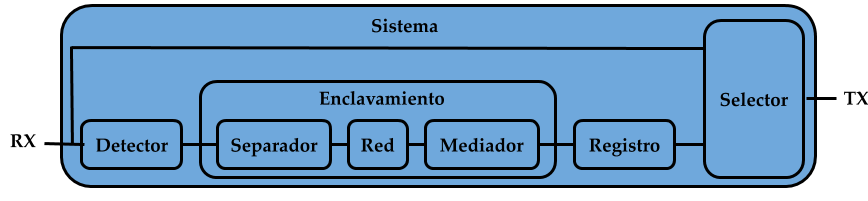
\includegraphics[scale=0.45]{./Figures/Diagrama_general}
		\caption{Diagrama general del sistema.}
		\label{fig:Diagrama_general}
	\end{figure}
	
	\vspace{2cm}
	
	Por simplicidad del diagrama, no se han incluido los bloques referidos a la UART que también son generados automáticamente. Tampoco se ha entrado en detalles respecto al interior del bloque "red", ya que el mismo presenta una cantidad variable de bloques "nodo" y "cambios", contados también de forma variable. Por lo que un diagrama no podría representarlo fielmente.
	
	Se ilustra en la figura \ref{fig:UART_General} la conexión entre el sistema y la computadora. La comunicación entre la computadora y la plataforma FPGA es posible gracias a una UART generada automáticamente. La misma adapta su tamaño según las tramas que necesita el sistema para funcionar.
	
	\begin{figure}[h]
	\centering
	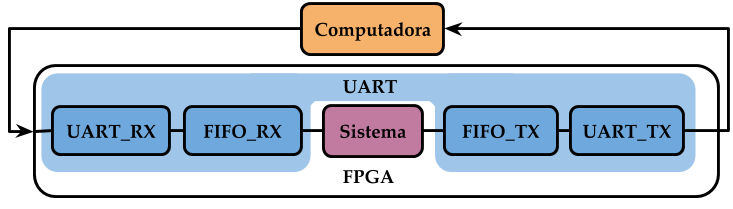
\includegraphics[scale=0.5]{./Figures/Diagrama_UART_PC}
		\caption{Diagrama de conexión del sistema a la computadora.}
		\label{fig:UART_General}
	\end{figure}
	
	Para poder verificar el funcionamiento del sistema a nivel general, primero es necesario verificar que cada bloque se comporta como debe. En la siguientes secciones se abordará la verificación de cada uno de los bloques.	
				
\section{Verificación de la implementación del nodo}

	La generación automática de código instancia, dentro del bloque ''red'', diferentes tipos de nodos, tal como se explicó en la sección \ref{nodos}. A la hora de realizar los ensayos de verificación de la implementación del nodo se utilizó como bloque de prueba el nodo mas completo, que corresponde al nodo perteneciente al tramo de vía que incluye la máquina de cambios. De esta forma se tiene la mayor cantidad de semáforos, interacciones, vecinos y comportamientos posibles.
	
	\subsection{Testbench del módulo nodo}
			
			Se diseñó un testbench para evaluar todas las posibles combinaciones de estados, definidas en la Tabla \ref{tabla_nodos}, además de la posición del cambio de vías próximo.
					
			\begin{table}[!hbt]
			\renewcommand{\arraystretch}{1.3}
			\caption{Combinaciones posibles}
			\label{tabla_nodos}
			\centering
			\begin{tabular}{ c  c  c }
			\hline
			Tramo propia & Tramo vecino & Aspecto vecino \\	
			\hline
			Ocupado & Ocupado & Rojo  \\
			Ocupado & Ocupado & Amarillo  \\
			Ocupado & Ocupado & Verde  \\	
			Ocupado & Libre & Rojo  \\
			Ocupado & Libre & Amarillo  \\
			Ocupado & Libre & Verde  \\	
			Libre & Ocupado & Rojo  \\
			Libre & Ocupado & Amarillo  \\
			Libre & Ocupado & Verde  \\	
			Libre & Libre & Rojo  \\
			Libre & Libre & Amarillo  \\
			Libre & Libre & Verde  \\	
			\end{tabular}
			\end{table}	
	
		Los semáforos asociados al nodo deberán pasar a un aspecto rojo cuando la posición del cambio o la ocupación de su sección o la sección vecina impidan el movimiento del tren sin colisionar o descarrillar. Para las demás combinaciones, el aspecto dependerá de la ocupación y aspectos presentados por sus vecinos, para presentar el doble recubrimiento exigido por las normas ferroviarias, tal como se explicó en la sección \ref{CVs}.
			
		\subsection{Resultados obtenidos}
			
			En la figura \ref{fig:Test_Nodo} se muestra el resultado obtenido. Siempre que el tramo está ocupado el semáforo cambia su aspecto a rojo. Si el tramo analizado está desocupado se desprenden varios casos:
			
			\begin{itemize}
				\item Si el vecino esta ocupado: el semáforo analizado estará en aspecto rojo.
				\item Si el vecino está desocupado:
				\begin{itemize}
					\item Si el semáforo vecino está en rojo: el semáforo analizado estará en aspecto amarillo.
					\item Si el semáforo vecino está en amarillo:  el semáforo analizado estará en aspecto verde.
				\end{itemize}				 
			\end{itemize}
			
			\begin{figure}[h]
			\centering
			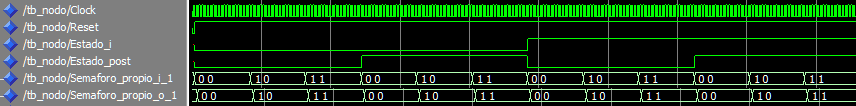
\includegraphics[scale=0.6]{./Figures/Test/Nodo}
				\caption{Simulación de un nodo.}
				\label{fig:Test_Nodo}
			\end{figure}
				
			El haber validado el nodo genérico que incluye todos los posibles estados que pueden tener los nodos más simples, se considera que el ensayo fue exitoso.	
	
\section{Verificación de la implementación de la máquina de cambios}

	El módulo de la máquina de cambios, incluido dentro del bloque ''red'', tiene como función el conectar al estado anterior con el estado posterior o al estado anterior con el estado desvío según la posición del cambio de vías, como se indica en la Tabla \ref{tabla_cambios}.
	
			\begin{table}[!hbt]
			\renewcommand{\arraystretch}{1.3}
			\caption{Combinaciones posibles}
			\label{tabla_cambios}
			\centering
			\begin{tabular}{ c  c  c  c}
			\hline
			Posición del cambio & Estado anterior & Estado posterior & Estado desvío \\	
			\hline
			Normal & Ocupado & Ocupado  & Ocupado \\
			Normal & Ocupado & Ocupado  & Libre \\
			Normal & Ocupado & Libre  & Ocupado \\
			Normal & Ocupado & Libre  & Libre \\
			Normal & Libre & Ocupado  & Ocupado \\
			Normal & Libre & Ocupado  & Libre \\
			Normal & Libre & Libre  & Ocupado \\
			Normal & Libre & Libre  & Libre \\
			Inversa & Ocupado & Ocupado  & Ocupado \\
			Inversa & Ocupado & Ocupado  & Libre \\
			Inversa & Ocupado & Libre  & Ocupado \\
			Inversa & Ocupado & Libre  & Libre \\
			Inversa & Libre & Ocupado  & Ocupado \\
			Inversa & Libre & Ocupado  & Libre \\
			Inversa & Libre & Libre  & Ocupado \\
			Inversa & Libre & Libre  & Libre \\	
			\end{tabular}
			\end{table}	
	
	\subsection{Testbench del módulo de la máquina de cambios}
			
		Se diseñó un testbench donde se ensayan todas las combinaciones definidas en la Tabla \ref{tabla_cambios} para una topología de medio bypass con un único cambio, para simplificar la presentación de los resultados.
						
	\subsection{Resultados obtenidos}
			
		En la figura \ref{fig:Test_Cambios} se visualizan los resultados del ensayo. Cuando la posición de la máquina de cambios es normal entonces el estado anterior y el posterior están comunicados y cada uno puede ver tanto la ocupación como los semáforos del otro. Cuando la posición de la máquina de cambios es inversa entonces los estados vinculados son el anterior y el estado del nodo perteneciente al desvío.
		
		\begin{figure}[h]
		\centering
		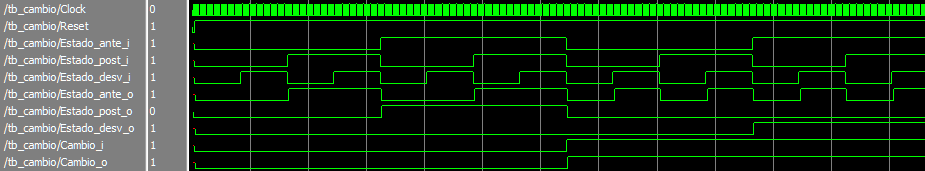
\includegraphics[scale=0.55]{./Figures/Test/Cambio}
			\caption{Simulación de la máquina de cambios.}
			\label{fig:Test_Cambios}
		\end{figure}
			
		\vspace{5cm}
			
		El nodo de cambios funciona de manera sincrónica y se comprobó que vincula correctamente los estados de los nodos involucrados. A diferencia de los bloques de nodos donde todos los nodos implementados tienen la misma cantidad de funciones que el ensayado o menor, todos los cambios tienen las mismas funcionalidades sin ninguna limitación, por lo que este ensayo es representativo del conjunto de máquinas de cambios y es suficiente para validar su correcto funcionamiento.
				
\section{Verificación de la implementación de la UART}

	En el diseño del sistema se contempló utilizar uno de los switches de la placa de desarrollo para poder puentear todo el enclavamiento y probar fácilmente el funcionamiento de la UART sin el efecto del enclavamiento. En esta sección se realizó el ensayo con el switch en la posición en la cual la salida recibe el mensaje de la entrada directamente, sin pasar por ningun otro bloque.

	\subsection{Testbench del módulo UART}
			
		Se diseñó un testbench en el cual se inyecta la entrada de la UART directamente a la salida de la UART, teniendo una prueba de bucle cerrado. Todos los mensajes ingresados, siempre que sean válidos, pasarán a la salida para ser publicados en la terminal desde donde se originaron.
						
	\subsection{Resultados obtenidos}
				
		En la figura \ref{fig:Test_UART} se presentan los datos obtenidos en el ensayo. Se puede ver que las tramas inyectadas son presentadas idénticamente en la salida, con un pequeño delay temporal. Además de poder apreciar el tren de pulsos que envía la UART de un extremo al otro del módulo, primero para indicar la lectura de la FIFO de recepción y luego para indicar la escritura de la FIFO de transmisión.
		
		\begin{figure}[h]
		\centering
		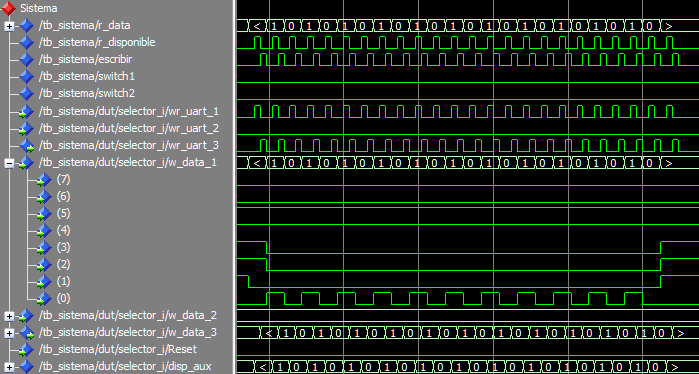
\includegraphics[scale=0.7]{./Figures/Test/UART}
			\caption{Simulación de la UART.}
			\label{fig:Test_UART}
		\end{figure}
			
		\vspace{10cm}
			
		Solo después de superado este ensayo se pudo avanzar con la inclusión de los demás módulos. Esto se debe a que no tenía sentido implementar sistemas complejos sin la certeza de que la transmisión y recepción de datos de la computadora a la plataforma era fiable. %Este proceso de desarrollo requirió varias iteraciones por la dificultad que implicó depurar cada uno de los elementos involucrados.
	
\section{Verificación de la implementación del detector}

	El bloque detector tiene como función descartar todas las tramas que no cumplan con el requisito definido de poseer tag inicial y final, además de que el mensaje debe tener una cantidad de elementos indicado por la UART.
	
	Para probar el sistema se deberán enviar:
	
	\begin{itemize}
		\item Tramas con tags incorrectos
		\item Tramas con ausencia de alguno o ambos tags
		\item Tramas con menos datos de los indicados
		\item Tramas con mas datos de los indicados
		\item Tramas correctas de elementos nulos, con un solo elemento válido en todas las posiciones posibles.
	\end{itemize}
	
	\subsection{Testbench del módulo detector}
			
		Se diseñó un testbench que inyecta las señalas necesarias para probar la detección de las tramas correctas y el descarte de las incorrectas. Además deberá envíar las señales de activación/desactivación de las próximas etapas, así como recibir las señales inhibidoras necesarias. Por una cuestión de espacio se recortó parte del algoritmo presentado.		
						
	\subsection{Resultados obtenidos}
				
		En la figura \ref{fig:Test_Detector} se puede visualizar una parte de los resultados del ensayo. Este ensayo corresponde al envío de cuatro paquetes distintos y el módulo va alternando los estados según el evento ocurrido. 
		
		\begin{figure}[h]
		\centering
		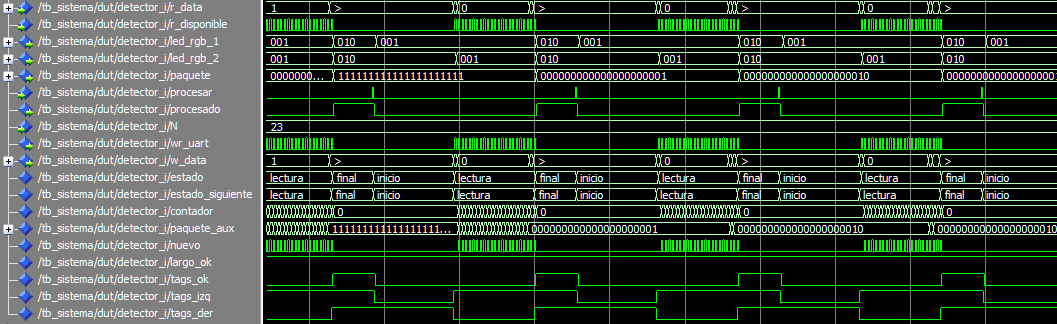
\includegraphics[scale=0.5]{./Figures/Test/Detector}
			\caption{Simulación del detector.}
			\label{fig:Test_Detector}
		\end{figure}

		Cuando se recibe el tag inicial ('<') el sistema pasa al estado de lectura y debe recibir la cantidad de elementos indicada por la señal N (en este caso 23). El elemento número 24 leído deberá ser el tag final('>'), que al recibirlo se pasa al estado final (en caso contrario pasa al estado error) a la espera de que la transmisión termine.
		
		Para la transmisión, cada caracter (byte) leído deberá ser convertido en un booleano (bit) para ser empaquetado en un vector de booleanos. Esto puede verse en la señal auxiliar paquete\_aux que luego de validada toda la trama se envía por w\_data al próximo bloque, junto con el tren de pulsos wr\_uart para indicar el ciclo de lectura de la señal.
		
		El ensayo fue exitoso y todas las tramas listadas como erróneas al comienzo del ensayo fueron descartadas de acuerdo a lo previsto.
		
\section{Verificación de la implementación del enclavamiento}	

	Utilizando el mismo algoritmo que para validar la UART, pero con el switch en la posición contraria, se pueden enviar las señales del módulo detector al enclavamiento. De esta forma se pueden probar los bloques separador, enclavamiento y mediador.
	
	\subsection{Testbench del módulo enclavamiento}
			
		Se diseñó un testbench para ensayar los módulos mencionados. En este caso se inyectan diferentes señales para comprobar que el módulo separador puede justamente separar las señales en vectores manejables. Luego de ser procesados por el enclavamiento, las señales son enviadas al mediador para volver a unificarlas en una sola señal. Finalmente el registro convierte cada elemento de la señal en un caracter imprimible que será enviado a la UART.		
						
	\subsection{Resultados obtenidos}
				
		En la figura \ref{fig:Test_Separador} se puede visualizar como la trama principal es separada en los diferentes vectores que serán recibidos por el enclavamiento. La separación es exitosa al ser un módulo de cuya dificultad radicaba en su automatización, mas no en su funcionamiento. El haber separado esta funcionalidad del resto del enclavamiento fue beneficioso para todo el diseño.
		
		\begin{figure}[!hbt]
		\centering
		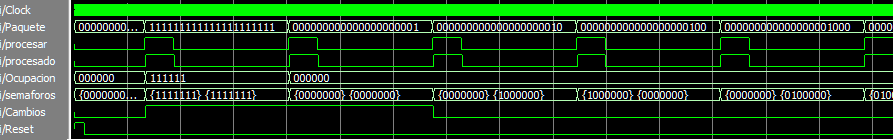
\includegraphics[scale=0.55]{./Figures/Test/Separador}
			\caption{Simulación del separador.}
			\label{fig:Test_Separador}
		\end{figure}
		
		En la figura \ref{fig:Test_Enclavamiento} se visualiza el comportamiento del enclavamiento ante las señales que fueron enviadas por el separador. En base al aspecto de los semáforos relevados en campo (sem\_s\_i) y a la ocupación de los tramos de vías (cv\_s) el enclavamiento determina que el aspecto de los semáforos para que no ocurran colisiones ni descarrilamientos es el que indica en la señal sem\_s\_o.
		
		\begin{figure}[!hbt]
		\centering
		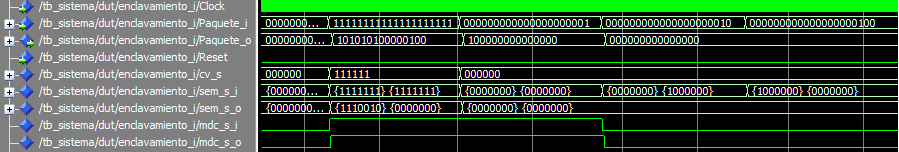
\includegraphics[scale=0.7]{./Figures/Test/Enclavamiento}
			\caption{Simulación del enclavamiento.}
			\label{fig:Test_Enclavamiento}
		\end{figure}

		%\vspace{5cm}
		
		En la figura \ref{fig:Test_Mediador} se presenta el proceso inverso del módulo mediador, donde las señales del enclavamiento son combinadas en una única señal.
		
		\begin{figure}[!hbt]
		\centering
		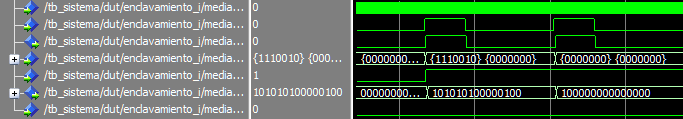
\includegraphics[scale=0.9]{./Figures/Test/Mediador}
			\caption{Simulación del mediador.}
			\label{fig:Test_Mediador}
		\end{figure}
		
		Los módulos separador, enclavamiento y mediador son parte de un módulo mayor, al funcionar los tres correctamente se ha comprobado que también funciona de forma el bloque que los integra.
		
\section{Verificación de la implementación del registro}

	El módulo de registro tiene la función de recibir una señal de M elementos booleanos y devolver M caracteres que correspondan al valor del vector en cuestión. Además de generar un tren de pulsos para coordinar la correcta escritura de los caracteres en la UART para su posterior impresión en la consola.
	
	\subsection{Testbench del módulo registro}
			
		Se diseñó un testbench en el cual se ingresan diferentes tramas y se comprueba que a la salida se obtenga la secuencia de caracteres esperada.		
			
	\subsection{Resultados obtenidos}
				
		En la figura \ref{fig:Test_Registro} se visualiza el resultado del ensayo, para una trama aleatoria.
		
	\begin{figure}[h]
	\centering
	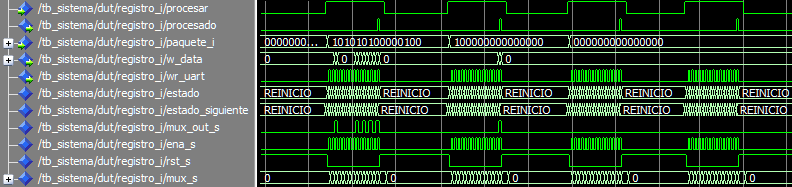
\includegraphics[scale=0.6]{./Figures/Test/Registro}
		\caption{Simulación del registro.}
		\label{fig:Test_Registro}
	\end{figure}
	
	Cuando la señal procesar se encuentra en alto, la señal paquete\_i es invertida y en cada ciclo ena\_s se envía el caracter equivalente al elemento del paquete\_i en la posición mux\_s. A su vez la señal ena\_s se envía a la UART a través de wr\_uart para indicarle el ciclo de escritura en la FIFO.
	
	Al finalizar la operación se envía la señal procesado para indicarle al bloque detector que el paquete ingresado ya ha sido enviado, de forma tal de iniciar otro ciclo de lectura y procesamiento. De esa forma la señal procesar pasa a un estado bajo a la espera de dicha lectura.
	
	El comportamiento del bloque fue tal cual fue diseñado y responde con un delay muy bajo de 2 ciclos de reloj. Por lo que tendríamos un espaciado entre tramas de hasta un mínimo de 16 nanosegundos, lo cual es muy positivo a la hora de tener un sistema que debe responder de forma rápida a los cambios en el exterior.	
	
\section{Verificación de la implementación del selector}

	Al módulo selector pueden llegar señales por dos caminos: directamente desde el módulo detector la señal de entrada sin procesar junto con su tren de pulsos asociado o la mismas señales pero procesadas previamente por el sistema de enclavamiento. Es tarea del módulo selector el enviar a la UART las señales de una u otra fuente, según la posición del switch.	
	
	\subsection{Testbench del módulo selector}
			
		Se diseñó un testbench que inyecta dos señales idénticas, una mientras el switch se encuentra en posición alta y otra mientras se encuentra en posición baja.		
						
	\subsection{Resultados obtenidos}
				
		En la figura \ref{fig:Test_Selector} se visualiza el comportamiento del sistema con el switch en estado alto. Se puede comprobar que ambas señales llegan al módulo: w\_data\_1 y wr\_uart\_1 son la señal con información y el tren de pulsos que corresponden a no procesar la señal; mientras que w\_data\_2 y wr\_uart\_2 son las mismas pero luego de haber sido procesadas por el sistema de enclavamiento.
			
	\begin{figure}[h]
	\centering
	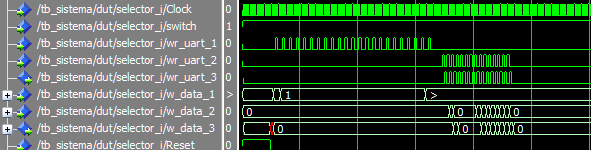
\includegraphics[scale=0.9]{./Figures/Test/Selector}
		\caption{Simulación del selector.}
		\label{fig:Test_Selector}
	\end{figure}
	
	\vspace{5cm}
			
	Las señales w\_data\_3 y wr\_uart\_3 son la salida del bloque selector, que se puede apreciar copian exactamente a w\_data\_2 y wr\_uart\_2. Cuando el switch se encuentra en estado bajo la salida copiará a w\_data\_1 y wr\_uart\_1.
	
\section{Prueba de integración: topología bypass.}

	Finalmente se realizó una prueba de integración sobre una topología topología bypass, que se muestra en la figura \ref{fig:Bypass_1}.

	\begin{figure}[h]
	\centering
	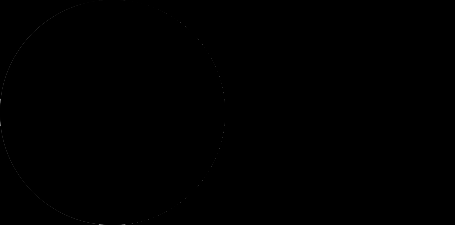
\includegraphics[scale=0.5]{./Figures/XXX}
		\caption{Topología bypass sin procesar.}
		\label{fig:Bypass_1}
	\end{figure}
	
	Una vez que la topología es analizada por el analizador de redes ferroviarias, se clasifican todos sus nodos y se determinan todos los semáforos. El resultado del análisis es presentado en la figura \ref{fig:Bypass_2}.

	\begin{figure}[h]
	\centering
	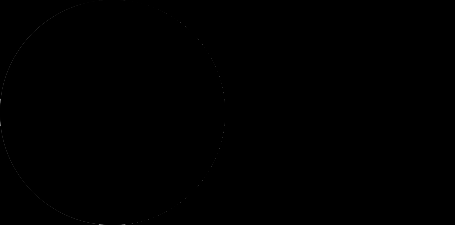
\includegraphics[scale=0.5]{./Figures/XXX}
		\caption{Topología bypass procesada.}
		\label{fig:Bypass_2}
	\end{figure}
	
	El programa utiliza todos los semáforos creados para generar todas las rutas soportadas por la topología. Además, sólo a los fines de poder hacer la comprobación manual, genera la tabla de enclavamientos, tal como se muestra en la Tabla \ref{tabla_bypass}.

	\begin{table}[!hbt]
	%\renewcommand{\arraystretch}{1.3}
	\caption{Tabla de enclavamientos de la topología bypass.}
	\label{tabla_bypass}
	\centering
	\begin{tabular}{ c  c  c  c  c }
	\hline
	Ruta & Semáforo inicial & Semáforo final & Secuencia & Sentido \\	
	\hline
		1 & 2 & 1 & 2-1 & < \\
		2 & 2 & 14 & 2-3-4-7-11-14 & > \\
	\end{tabular}
	\end{table}	
	
	Se generan los archivos de vhdl que describen el sistema, como se muestra en la figura \ref{fig:Bypass_3}.
	
	\begin{figure}[h]
	\centering
	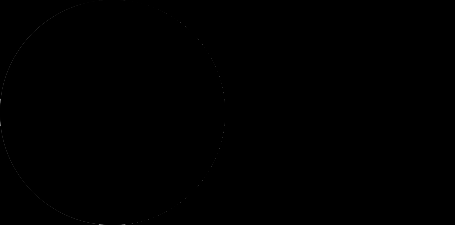
\includegraphics[scale=0.5]{./Figures/XXX}
		\caption{Archivos .VHDL generados.}
		\label{fig:Bypass_3}
	\end{figure}
	
	En base a dichos archivos .vhdl se crean todos los bloques necesarios para implementar el sistema en la plataforma FPGA. A modo de ejemplo se presenta en la figura \ref{fig:Bypass_4} las conexiones del bloque ''red''. En el mismo se muestran diez bloques de nodos y dos de máquinas de cambios. 
	
	\begin{figure}[h]
	\centering
	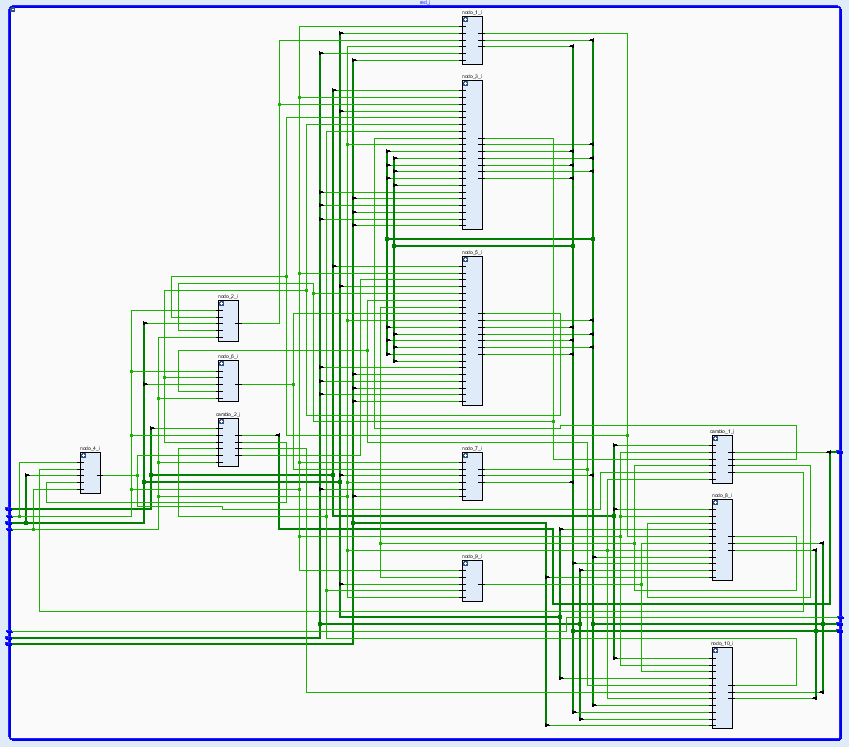
\includegraphics[scale=0.5]{./Figures/Red}
		\caption{Módulo de red generador.}
		\label{fig:Bypass_4}
	\end{figure}
	
	Los bloques de nodos tendrán diferentes tamaños según cómo fuesen clasificados por el analizador de redes ferroviarias. Los nodos que incluyen las máquinas de cambios (3 y 5) tendrán un tamaño mucho mayor que los nodos simples (2, 6 y 9).
	
	La densidad de conexiones es tan grande que queda de manifiesto la complejidad de realizar esta labor de forma manual. Haber desarrollado el analizador de redes ferroviarias, incluyendo la automatización de la generación de código, es una ventaja a la hora de abordar topologías mas complejas. Ya que la implementación se lleva a cabo sin elevar el tiempo de desarrollo ni incrementar las posibilidades de introducir errores humanos.
	
	Se establece una conexión serie entre la computadoray la plataforma FPGA por medio del analizador de redes ferroviarias. Se muestran en las figuras \ref{fig:Bypass_5} y \ref{fig:Bypass_6} el resultado de ocupar el nodo 3 y modificar la posición de las máquinas de cambios respectivamente.
	
	\begin{figure}[h]
	\centering
	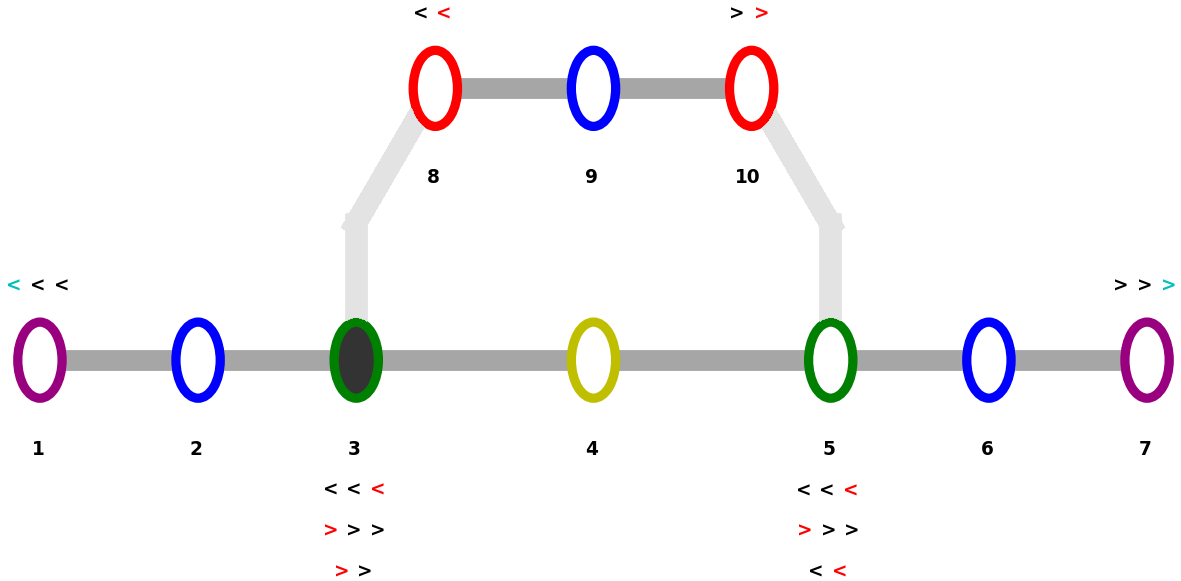
\includegraphics[scale=0.5]{./Figures/Mapa_A}
		\caption{Bypass con circulación normal y nodo 3 ocupado.}
		\label{fig:Bypass_5}
	\end{figure}

	\begin{figure}[h]
	\centering
	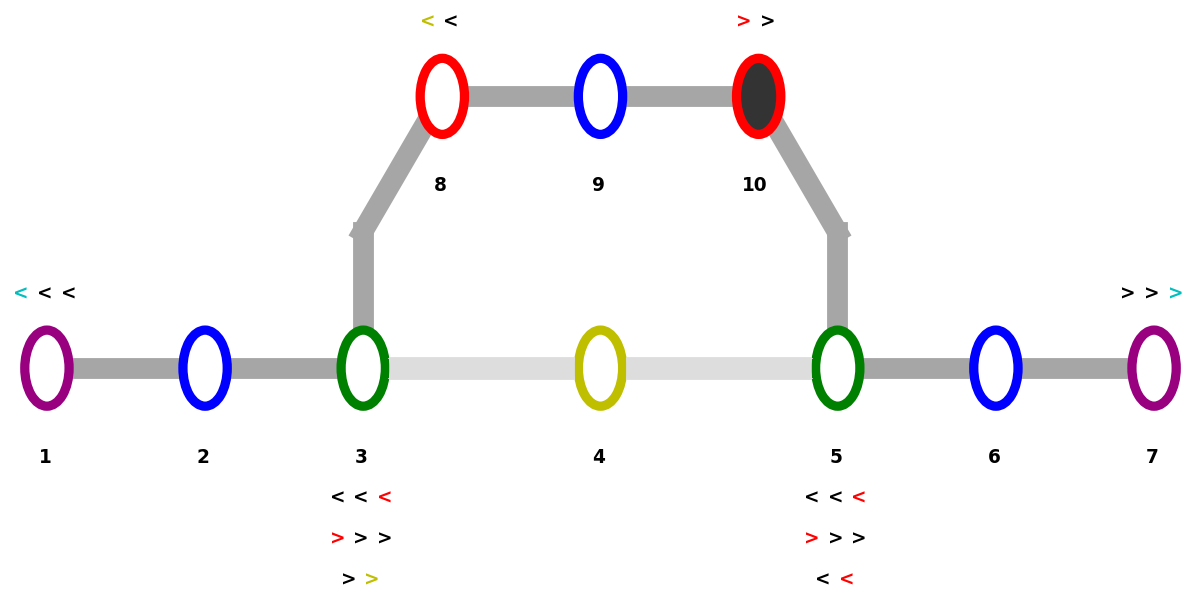
\includegraphics[scale=0.5]{./Figures/Mapa_B}
		\caption{Bypass con circulación inversa y nodo 10 ocupado.}
		\label{fig:Bypass_6}
	\end{figure}
	
	
	-ANALISIS FINAL DE AMBAS IMAGENES
	

	De esta forma concluye este capítulo, en el cual se presentaron los ensayos realizados y los resultados obtenidos.
